\section{Experiment 10F: control-relevance stress test}
\label{sec:experiment10f}

\paragraph{Motivation and claim gate.}
Experiment 10E reduced full-envelope matrix error by 23.74\% relative to
Global, but its isolated recovery metric improved by only 0.031\%. Better
identification therefore did not yet imply a practically distinguishable
control result. Experiment 10F tests the missing link under nonlinear,
speed-varying yaw-rate tracking with actuator constraints. A valid
control-relevance claim requires FederatedLearned to improve over Global on
fresh fleets after the maneuver and controller have been frozen without using
their pairwise result.

\paragraph{Controller audit without method-directed tuning.}
Twelve LQI configurations vary sideslip, yaw-rate, and integral weights and the
steering penalty. On development fleets 381--385, every configuration is
evaluated using only each client's ExactLPV model. Neither Global nor
FederatedLearned is evaluated during selection. A candidate must retain
feasibility on every development trajectory, have less than 5\% mean actuator
saturation, and satisfy the dense-grid small-signal stability test. Among
passing candidates, the controller with minimum mean ExactLPV tracking RMSE is
selected. The frozen choice is
\begin{equation}
 Q=\operatorname{diag}(25,50,1000),\qquad R=0.15.
\end{equation}
All twelve candidates pass the constraints. The selected controller obtains
0.0954~deg/s mean tracking RMSE across the two development maneuvers, compared
with 0.1818~deg/s for the most conservative candidate.

An initial maneuver-intensity pilot on seeds 391--400 is excluded from all
reported confirmation results. That pilot produced only about 2~deg/s peak
steering rate, no saturation, and approximately 0.01~deg/s tracking error. It
therefore did not constitute a meaningful stress test. The final protocol was
redefined using physically interpretable lateral-acceleration requests, and a
new untouched confirmation set was reserved.

\paragraph{Final protocol.}
Confirmation uses ten fresh fleets (seeds 411--420), globally randomized
label-free coverage, and the complete federated latent-group estimator from
Experiment 10E. The reference curvature is generated as
\begin{equation}
 \kappa_{\mathrm{ref}}(t)=\frac{a_{y,\mathrm{ref}}(t)}{v(t)^2},
 \qquad r_{\mathrm{ref}}(t)=v(t)\kappa_{\mathrm{ref}}(t),
\end{equation}
which prevents speed variation from accidentally changing maneuver severity.
The moderate multisine requests up to approximately 4~m/s$^2$. The hard
three-pulse maneuver requests up to approximately 7~m/s$^2$, close to the
nonlinear tire envelope. Both use smooth speed profiles spanning 11--29~m/s or
12--29~m/s.

At each sample, the controller interpolates the scheduled LQI gain and
prefilter from the eleven design speeds. Steering is limited to 12~deg and
120~deg/s. Conditional integration prevents windup. Feasibility requires
finite trajectories and peak sideslip below 6~deg. We report mean and
worst-client yaw-rate tracking RMSE, peak tracking error, sideslip, steering,
saturation, and the maximum dense-grid spectral radius. Local retains the
conservative nearest-observed-speed rule outside its local block.

\begin{table}[htbp]
\centering
\caption{Experiment 10F confirmation results. Tracking values are yaw-rate
RMSE in deg/s, averaged across ten fresh fleets.}
\label{tab:experiment10f-summary}
\begin{tabular}{llrrrr}
\toprule
Maneuver & Method & Mean & Worst client & Feasible & $\rho_{\max}$\\
\midrule
Moderate & Local            & 0.05396 & 0.08870 & 10/10 & 0.9761\\
Moderate & Global           & 0.04290 & 0.05637 & 10/10 & 0.9756\\
Moderate & FederatedLearned & 0.04108 & 0.05303 & 10/10 & 0.9759\\
Moderate & ExactLPV         & 0.04002 & 0.04072 & 10/10 & 0.9759\\
\midrule
Hard & Local                & 0.16981 & 0.21845 & 10/10 & 0.9761\\
Hard & Global               & 0.15644 & 0.18317 & 10/10 & 0.9756\\
Hard & FederatedLearned     & 0.15457 & 0.17714 & 10/10 & 0.9759\\
Hard & ExactLPV             & 0.15074 & 0.16332 & 10/10 & 0.9759\\
\bottomrule
\end{tabular}
\end{table}

\begin{table}[htbp]
\centering
\caption{Paired FederatedLearned improvements over Global. Positive values
favor FederatedLearned. Absolute changes are in deg/s.}
\label{tab:experiment10f-global}
\begin{tabular}{llrrr}
\toprule
Maneuver & Metric & Relative & 95\% CI & Absolute\\
\midrule
Moderate & Mean tracking  & 4.26\% & [1.95,6.55]\% & 0.00182\\
Moderate & Worst client   & 5.90\% & [1.03,11.20]\% & 0.00335\\
Hard     & Mean tracking  & 1.21\% & [0.47,2.01]\% & 0.00187\\
Hard     & Worst client   & 3.31\% & [1.16,5.77]\% & 0.00603\\
\bottomrule
\end{tabular}
\end{table}

\begin{figure}[htbp]
\centering
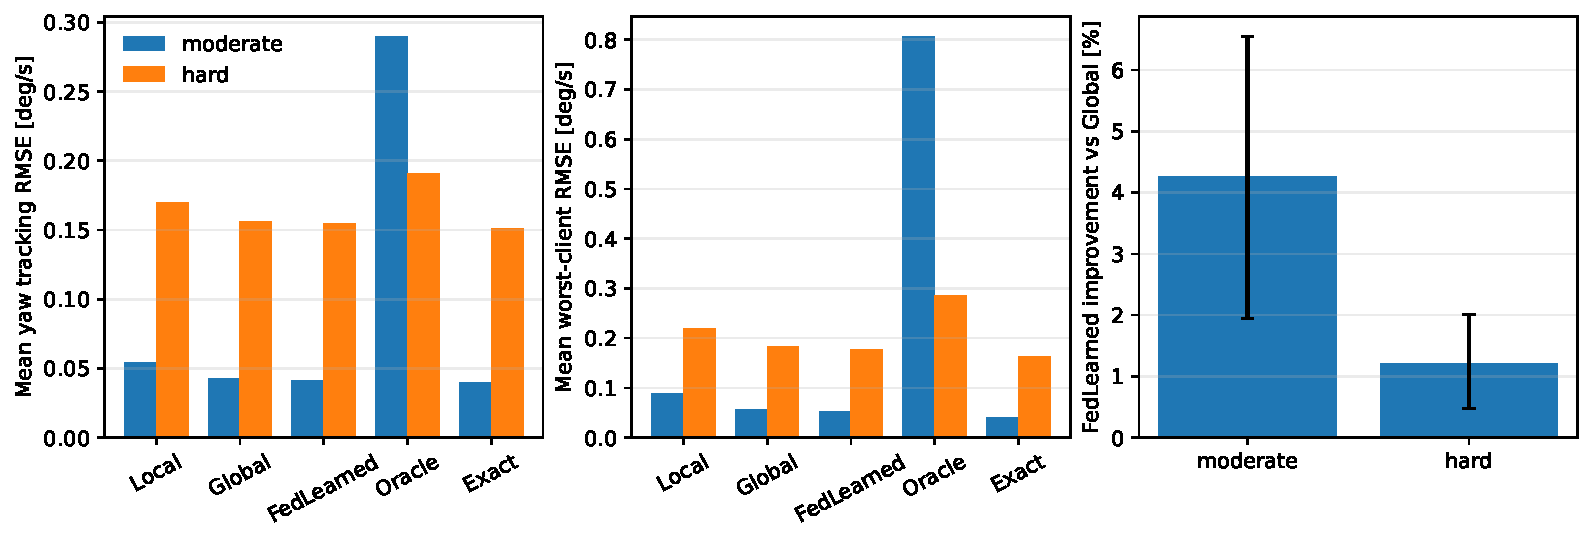
\includegraphics[width=0.98\linewidth]{../results/figures/experiment_10f_control_relevance.pdf}
\caption{Experiment 10F mean and worst-client tracking under the frozen
controller, with paired improvement of FederatedLearned over Global.}
\label{fig:experiment10f}
\end{figure}

\paragraph{Result.}
The predeclared control-relevance gates pass. FederatedLearned improves mean
tracking relative to Global by 4.26\% in the moderate maneuver and 1.21\% in
the hard maneuver. The paired 95\% intervals are positive. Worst-client
tracking improves by 5.90\% and 3.31\%, respectively, also with positive
intervals. FederatedLearned improves over restricted Local by 23.86\% in the
moderate maneuver and 8.96\% in the hard maneuver. Every federated trajectory
is feasible, and the maximum scheduled small-signal spectral radius is 0.9759.

BIC selects two groups in six confirmation fleets and one group in four. In the
single-group fleets, FederatedLearned and Global are identical. Accordingly,
the six positive fleet-level differences against Global occur exactly where
the selector retains two groups. Across all fleets, learned grouping closes
63.3\% of the mean Global-to-Exact tracking gap in the moderate maneuver and
32.9\% in the hard maneuver. For worst-client tracking it closes 21.4\% and
30.4\%, respectively.

\paragraph{Critical interpretation.}
Experiment 10F establishes that the improved LPV models can propagate into
statistically supported closed-loop benefits under a frozen, independently
selected controller. It therefore resolves the binary control-relevance gate.
The practical magnitude relative to Global remains small: the mean absolute
improvements are only 0.00182 and 0.00187~deg/s. The paper may claim a
repeatable control effect and a meaningful fraction of the remaining
Global-to-Exact gap, but should not claim a large practical tracking gain.

The physical-family oracle is not uniformly reliable under label-free
coverage. In one confirmation fleet its pooled observations do not identify a
stable full-envelope scheduled controller, producing a maximum spectral radius
above three. This reinforces the Experiment 10E conclusion that compatibility
must account for information coverage as well as physical family membership.

\paragraph{Decision.}
The evidence chain now supports a genuine FL-and-control paper: local speed
blocks are individually insufficient, federated latent grouping reconstructs
full-envelope LPV models without labels, and the model improvement produces a
confirmed closed-loop benefit over both Local and Global. Before manuscript
consolidation, the remaining high-value robustness test is partial
participation or missing-block participation under the frozen 10F controller.
This should be treated as a robustness extension, not as another attempt to
increase the reported control gap.

\paragraph{Reproducibility.}
The configuration and implementation are in
\path{code/config/experiment_10f.json} and
\path{code/experiments/experiment_10f_control_relevance.py}. The frozen
controller selection, discarded-pilot disclosure, development audit,
confirmation records, aggregate summaries, paired intervals, and provenance
hashes are stored under 
\path{results/tables}.
